\documentclass{beamer}

\mode<presentation>
{
  \usetheme{Goettingen}
  \usecolortheme{seahorse}
  \setbeamercovered{transparent}
}

\usepackage[english]{babel}
\usepackage[latin1]{inputenc}

\usepackage{graphicx}
\graphicspath{ {images/} }

\usepackage{times}
\usepackage[T1]{fontenc}

\setlength{\parskip}{1em}

\title{When is a\\ crystal graph\\ not\\ crystallographic?}

\author[Olaf Delgado]{Olaf Delgado-Friedrichs}

\date{Order!Order? --- Canberra 4 Dec 2019}

\begin{document}

\begin{frame}
  \titlepage
\end{frame}

\section{Too much symmetry}

\begin{frame}
  \begin{center}
    Answer: when it has ``too much symmetry''.

    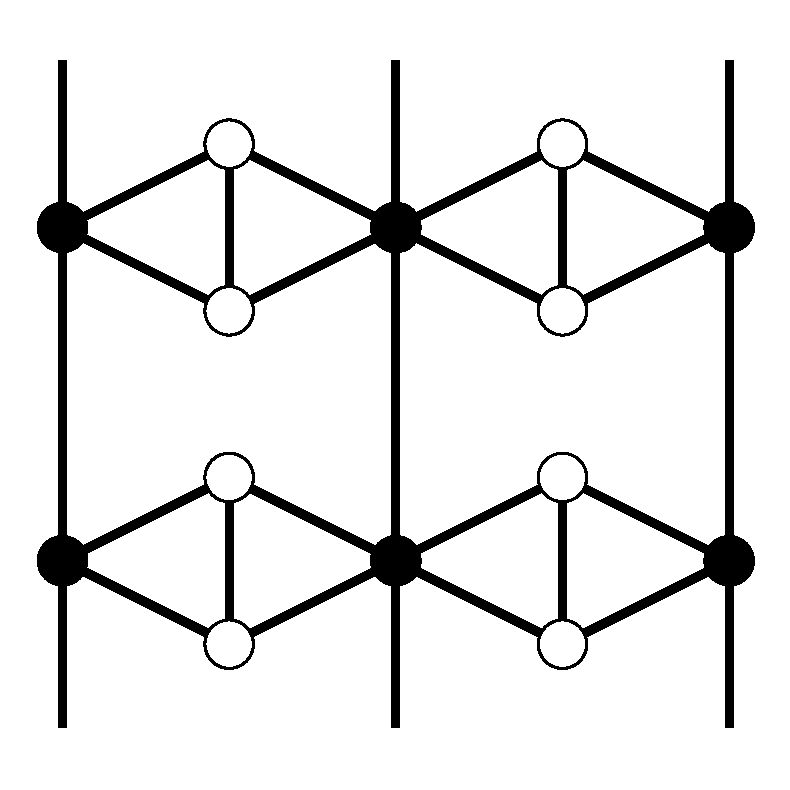
\includegraphics[width=1.7in]{unstable}
    \qquad
    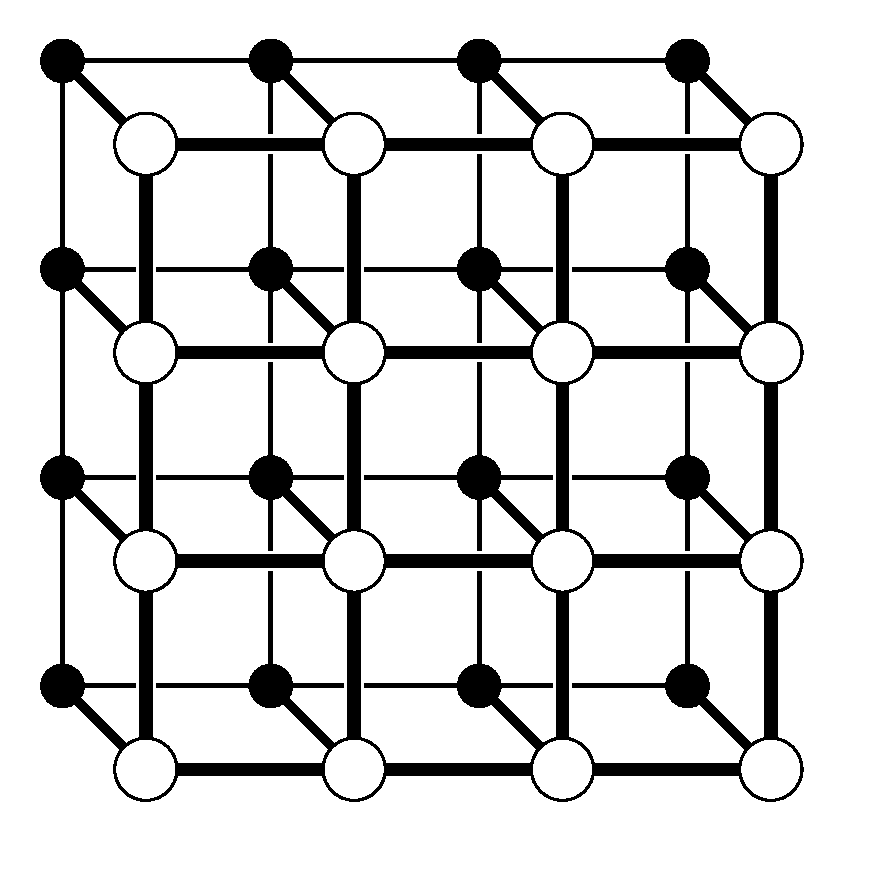
\includegraphics[width=1.7in]{ladder}

    More precisely: when its automorphism group is not a crystallographic
    space group.

    ({\em Crystallographic nets and their quotient graphs,}\\
    W.\ E.\ Klee 2004.)
  \end{center}
\end{frame}

\end{document}
